\section{Classification}
\index{Classification}

\noindent
\rule{7.0in}{.013in}

$Revision: 1.13 $

This section outlines classification methods of the {\marf} project.
First, we present you with the API and overall structure, followed
by the description of the methods. Overall structure of the modules
is in \xf{fig:classification}.

\begin{figure}
	\centering
	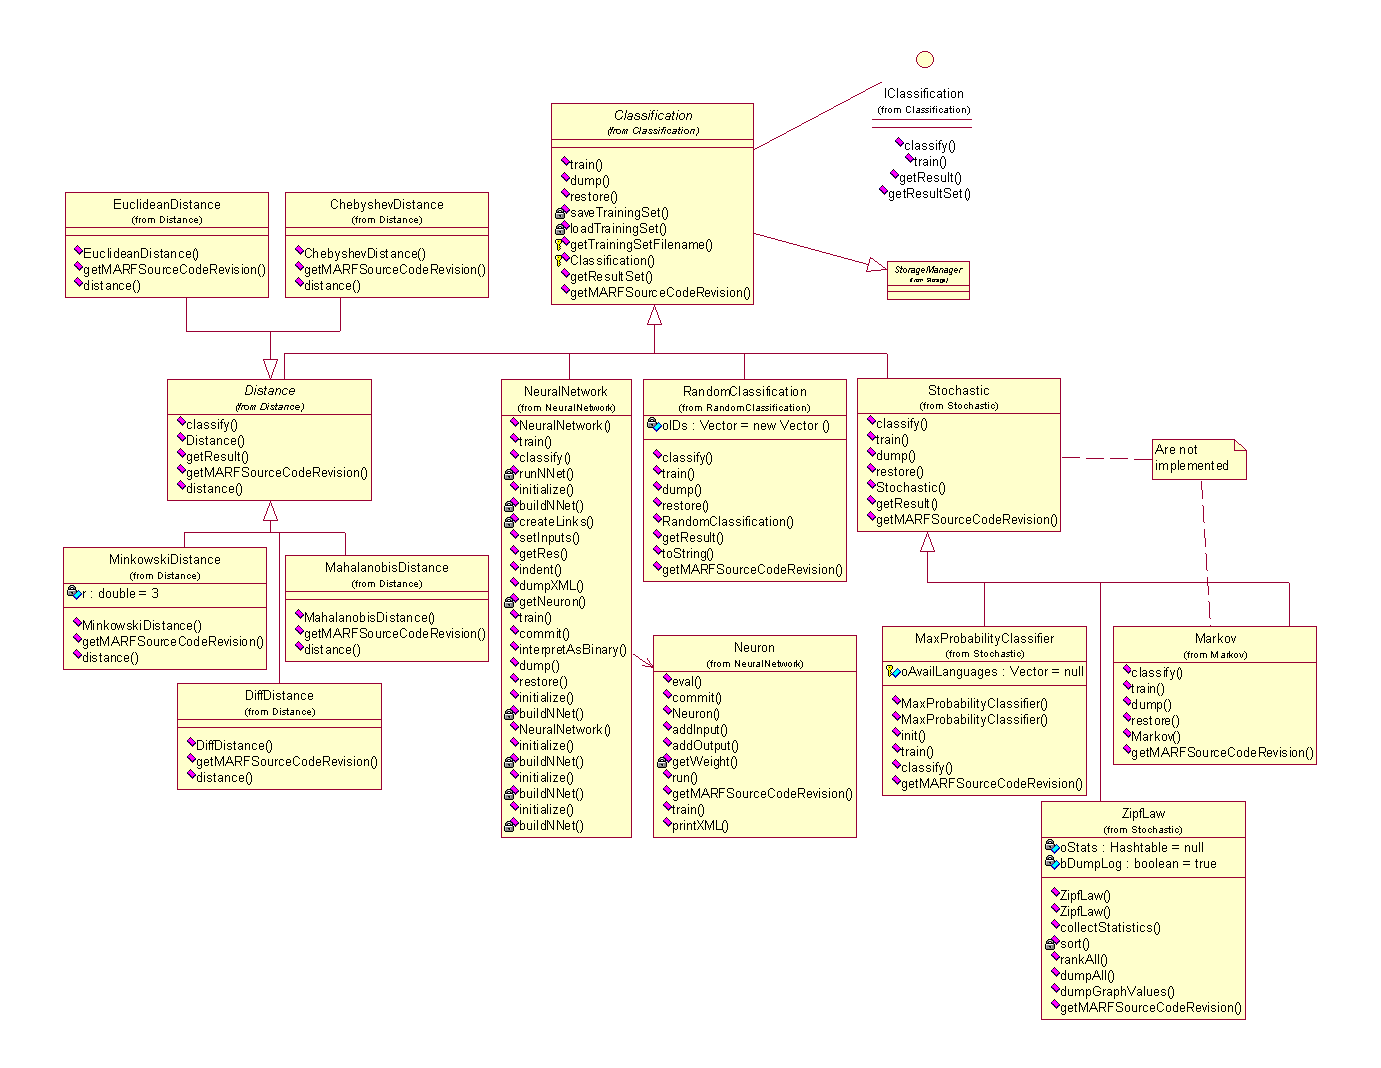
\includegraphics[angle=90,height=660pt]{../graphics/arch/classification.png}
	\caption{Classification}
	\label{fig:classification}
\end{figure}

\subsection{Chebyshev Distance}

Chebyshev distance is used along with other distance classifiers
for comparison. Chebyshev distance is also known as
a city-block or Manhattan distance. Here's its mathematical representation:

$$ d(x,y) = \displaystyle\sum_{k=1}^{n}(|x_{k}-y_{k}|) $$

\noindent
where $x$ and $y$ are feature vectors of the same length $n$.


\subsection{Euclidean Distance}

The Euclidean Distance classifier uses an Euclidean distance equation to find the
distance between two feature vectors.

If $A=(x_{1},x_{2})$ and $B=(y_{1},y_{2})$ are two 2-dimensional vectors, then the distance between
$A$ and $B$ can be defined as the square root of the sum of the squares of their
differences:

$$ d(x,y) = \sqrt{(x_{1}-y_{1})^{2} + {(x_{2}-y_{2})}^{2}} $$

This equation can be generalized to n-dimensional vectors by simply adding terms
under the square root.

$$ d(x,y) = \sqrt{(x_{n}-y_{n})^{2} + {(x_{n-1}-y_{n-1})}^{2} + ... + {(x_{1}-y_{1})}^{2}} $$

or

$$ d(x,y) = \sqrt{\displaystyle\sum_{k=1}^{n}(x_{k}-y_{k})^{2}} $$

or

$$ d(x,y) = \sqrt{(x-y)^{T}(x-y)} $$


A cluster is chosen based on smallest distance to the feature vector in question.


\subsection{Minkowski Distance}

Minkowski distance measurement is a generalization of both Euclidean
and Chebyshev distances.

$$ d(x,y) = \left(\displaystyle\sum_{k=1}^{n}(|x_{k}-y_{k}|)^{r}\right)^\frac{1}{r} $$

\noindent
where $r$ is a Minkowski factor. When $r=1$, it becomes Chebyshev distance,
and when $r=2$, it is the Euclidean one. $x$ and $y$ are feature vectors of the same length $n$.


\subsection{Mahalanobis Distance}
\label{sect:mahalanobis}
\index{Distance!Mahalanobis}
\index{Classification!Mahalanobis Distance}

$Revision: 1.7 $

\subsubsection{Summary}

\begin{itemize}
\item Implementation: \api{marf.Classification.Distance.MahalanobisDistance}
\item Depends on: \api{marf.Classification.Distance.Distance}
\item Used by: \api{test}, \api{marf.MARF}, \api{SpeakerIdentApp}
\end{itemize}

\subsubsection{Theory}

This distance classification is meant to be able to detect features
that tend to vary together in the same cluster if linear
transformations are applied to them, so it becomes invariant
from these transformations unlike all the other, previously seen
distance classifiers.

$$ d(x,y) = \sqrt{(x-y) C^{-1} (x-y)^{T}} $$

\noindent
where $x$ and $y$ are feature vectors of the same length $n$, and
$C$ is a covariance matrix, learnt during training for co-related
features.

In this release, namely 0.3.0-devel,
the covariance matrix being an identity matrix, $ C = I $,
making Mahalanobis distance be the same as the Euclidean one.
We need to complete the learning of the covariance matrix
to complete this classifier.

% EOF


\subsection{Diff Distance}
\label{sect:diff-distance}
\index{Distance!Diff}
\index{Classification!Diff Distance}

$Revision: 1.2 $

\subsubsection{Summary}

\begin{itemize}
\item Implementation: \api{marf.Classification.Distance.DiffDistance}
\item Depends on: \api{marf.Classification.Distance.Distance}
\item Used by: \api{test}, \api{marf.MARF}, \api{SpeakerIdentApp}
\end{itemize}

\subsubsection{Theory}

When Serguei Mokhov invented this classifier in May 2005, the original idea
was based on the way the \tool{diff} UNIX utility works. Later, for
performance enhancements it was modified. The essence of the diff distance is to
count how one input vector is different from the other in terms of
elements correspondence. If the Chebyshev distance between the two
corresponding elements is greater than some error $e$, then this
distance is accounted for plus some additional distance penalty $p$
is added. Both factors $e$ and $p$ can vary depending on desired
configuration. If the two elements are equal or pretty close
(the difference is less than $e$) then a small ``bonus'' of $e$ is subtracted
from the distance.

$$ d(x,y) = \sum_{i}{|x_i-y_i| + p, \mathit{if} |x_i-y_i| > e, \mathit{or} (-e)} $$

\noindent
where $x$ and $y$ are feature vectors of the same length.

% EOF


\subsection{Artificial Neural Network}
\label{sect:nnet}
\index{Artificial Neural Network}
\index{Neural Network}
\index{Methodology!Artificial Neural Network}
\index{Methodology!Neural Network}
\index{Algorithm!Artificial Neural Network}
\index{Algorithm!Neural Network}


This section presents implementation of the Neural Network Classification module.

One method of classification used is an Artificial Neural
Network. Such a network is meant to represent the neuronal
organization in organisms. Its use as a classification method lies is
in the training of the network to output a certain value given a
particular input \cite{artificialintelligence}.

\subsubsection{Theory}

A neuron consists of a set of inputs with associated weights, a
threshold, an activation function ($f(x)$) and an output value. The
output value will propagate to further neurons (as input values) in
the case where the neuron is not part of the ``output'' layer of the
network. The relation of the inputs to the activation function is as
follows:

$output \longleftarrow f(in)$

where $in = \displaystyle\sum_{i=0}^{n}(w_{i} \cdot a_{i}) - t$, ``vector'' $a$ is the
input activations, ``vector'' $w$ is the associated weights and $t$ is the
threshold of the network. The following activation function was used:

$sigmoid(x; c) = \frac{1}{(1 + e^{-cx})}$

where $c$ is a constant. The advantage of this function is that it is
differentiable over the region $(-\infty,+\infty)$ and has derivative:

$\frac{d(sigmoid(x; c))}{dx} = c \cdot sigmoid(x; c) \cdot (1 - sigmoid(x; c))$

The structure of the network used was a Feed-Forward Neural
Network. This implies that the neurons are organized in sets,
representing layers, and that a neuron in layer $j$, has inputs from
layer $j-1$ and output to layer $j+1$ only. This structure facilitates the
evaluation and the training of a network. For instance, in the
evaluation of a network on an input vector $I$, the output of neuron in
the first layer is calculated, followed by the second layer, and so
on.

\subsubsection{Training}

Training in a Feed-Forward Neural Network is done through the an
algorithm called Back-Propagation Learning. It is based on the error
of the final result of the network. The error the propagated backward
throughout the network, based on the amount the neuron contributed to
the error. It is defined as follows:

$w_{i,j} \longleftarrow \beta w_{i,j} + \alpha \cdot a_{j} \cdot \Delta_{i}$

where

$\Delta_{i} = Err_{i} \cdot \frac{df}{dx(in_{i})}$  for neuron $i$ in the output layer

and

$\Delta_{i} = \frac{df}{dt(in_{i})} \cdot \displaystyle\sum_{j=0}^{n}(\Delta_{j})$ for neurons in other layers

The parameters $\alpha$ and $\beta$ are used to avoid local minima in
the training optimization process. They weight the combination of the
old weight with the addition of the new change. Usual values for these
are determined experimentally.

The Back-Propagation training method was used in conjunction with
epoch training. Given a set of training input vectors $Tr$, the
Back-Propagation training is done on each run. However, the new weight
vectors for each neuron, ``vector'' $w'$, are stored and not used. After
all the inputs in $Tr$ have been trained, the new weights are committed
and a set of test input vectors $Te$, are run, and a mean error is
calculated. This mean error determines whether to continue epoch
training or not.

\subsubsection{Usage as a Classifier}

As a classifier, a Neural Network is used to map feature vectors to
speaker identifiers. The neurons in the input layer correspond to each
feature in the feature vector. The output of the network is the binary
interpretation of the output layer. Therefore the Neural Network has
an input layer of size $m$, where $m$ is the size of all feature vectors
and the output layer has size $\lceil(\log_{2}(n))\rceil$, where $n$ is the maximum
speaker identifier.

A network of this structure is trained with the set of input vectors
corresponding to the set of training samples for each speaker. The
network is epoch trained to optimize the results. This fully trained
network is then used for classification in the recognition process.

% EOF


\subsection{Random Classification}

That might sound strange, but we have a random classifier in {\marf}.
This is more or less testing module just to quickly test
the PR pipeline.  It picks an ID in the pseudo-random manner from the list of
trained IDs of subjects to classification.  It also serves as
a bottom-line of performance (i.e. recognition rate) for all
the other, slightly more sophisticated classification methods meaning
performance of the aforementioned methods must be better than
that of the Random; otherwise, there is a problem.


% EOF
